\subsection*{Genomic abundance of centromeric repeats}
Melters \textit{et al}. (2013) estimated that the medaka candidate centromeric satellite comprise 0.32\% of the medaka genome. However this estimation can underestimate the true genomic abundance due to its identification strategy. In order to better infer the genomic abundance of the centromeric satellite, PacBio raw reads were searched for the centromeric satellite sequence.

Genomic fraction of the centromeric repeat was estimated by searching PacBio subreads for the representative monomer sequence. The genomic fraction in Hd-rR and HNI genomes were estimated to be $\sim$1\%, while that in the HSOK genome was $\sim$2\% (Table \ref{centromeric_repeat_genomic_abundance}). This difference is consistent with the previous observations that centromeric repeat array size in a chromosome can vary up to 20-fold within a species \cite{Miga}. Assuming the genome size to be 800 Mb, the centromeric satellite comprise 8--16 Mb of the genome, which implies each chromosome has around 500 kb of centromeric satellite on average. This is concordant with the observations that the centromere of many higher eukaryotes studied to date are characterized by hundreds to thousands of kilobases of satellite sequences \cite{Plohl}. Although quantifying the centromeric satellite in erroneous PacBio reads can lead to slight underestimation, it provides much more reliable estimation than estimating by short Sanger sequencing reads.

\begin{table*}[htp]
  \centering
  \caption{Centromeric repeat genomic abundance}
  \begin{tabular}{p{1.5cm}p{2.5cm}p{3cm}p{3cm}p{3.5cm}p{2.5cm}}
  \hline
  strain & total subreads & passed subreads & passed subreads & repeats in passed subreads & estimated genomic abundance \\ \hline
  Hd-rR & 13,359,879 & 4,586,550 (34.33\%) & 34,933,754,979 bp & 354,930,731 bp (1.02\%) &  8.13 Mb \\
  HNI   & 14,777,797 & 7,265,969 (49.17\%) & 28,478,925,597 bp & 338,807,989 bp (1.19\%) &  9.52 Mb \\
  HSOK  &  5,527,528 & 1,955,979 (35.39\%) & 23,106,352,588 bp & 460,716,149 bp (1.99\%) & 15.95 Mb \\
  \hline
\end{tabular}

% \begin{tabulary}{18cm}{LRRRRR}
%   \hline
%   strain & total subreads & passed subreads & passed subreads & repeats in passed subreads & estimated genomic abundance \\ \hline
%   Hd-rR & 13,359,879 & 4,586,550 (34.33\%) & 34,933,754,979 bp & 354,930,731 bp (1.02\%) &  8.13 Mb \\
%   HNI   & 14,777,797 & 7,265,969 (49.17\%) & 28,478,925,597 bp & 338,807,989 bp (1.19\%) &  9.52 Mb \\
%   HSOK  &  5,527,528 & 1,955,979 (35.39\%) & 23,106,352,588 bp & 460,716,149 bp (1.99\%) & 15.95 Mb \\
%   \hline
% \end{tabulary}

  \label{centromeric_repeat_genomic_abundance}
  \caption*{\small{

  }}
\end{table*}


\subsection*{Centromeric repeat distribution}
The distribution of centromeric repeats in the three medaka strain genomes were revealed by searching their genomes using RepeatMasker (Table \ref{centromeric_repeat_distribution}). For those chromosomes that have $>$1 kb centromeric repeat, positions of the centromeres in chromosomes were classified, employing the nomenclature defined by Levan \textit{et al}. (1964) (Table \ref{centromeric_repeat_distribution}). Although the nomenclature was originally based on microscopic inspection of the centromeres in chromosomes rather than repeat distribution in the DNA sequence level, nevertheless the sequence-based classification conducted here is informative for inferring evolutionary relationship between the chromosomes. The composition of positional types were consistent with a previous karyotype study \cite{}. Centromeric positions of the same chromosome were mostly conserved among the strains, confirmed by observing the corresponding pair of genetic markers flanked the repeat arrays, with only two exceptions in chromosomes 4 and 6 (Supplementary figure S\ref{}). For chromosome 4, Hd-rR had an acrocentric repeat array whereas HSOK had a metacentric array. For chromosome 6, all the three strains had acrocentric repeat arrays but those of Hd-rR and HSOK and that of HNI were on the opposite side of the chromosome. As the karyotype study has revealed that the three strains possess slightly different sets of centromeric positions \cite{}, the difference of chromosomes 4 and 6 may be derived from the \textit{bona fide} karyotype difference. Of note, Hd-rR chromosome 21 possessed metacentric and acrocentric arrays of nearly the same length (41.6 kb and 45.5 kb, respectively; Supplementary figure S\ref{}), thus it may be a dicentric chromosome where one of the arrays forms the functional centromere whereas the other is silenced.

% TODO: prepare supplementary figure of centromeric positions shown in the genome browser.
% TODO: provide centromeric positions from the karyotype study as a supplementary table?

\begin{table*}[htp]
  \centering
  \caption{Centromeric repeat distribution}
  \begin{tabular}{r|rc|rc|rc}
  \hline
  & \multicolumn{2}{c|}{Hd-rR} & \multicolumn{2}{c|}{HNI} & \multicolumn{2}{c}{HSOK} \\ \hline
  chromosome & total repeat (bp) & position & total repeat (bp) & position & total repeat (bp) & position \\ \hline
  1  & 48,805  & SM  & 0      & -  & 0       & -  \\
  2  & 54,844  & M   & 3,831  & M  & 64,213  & M  \\
  3  & 52,681  & ST  & 0      & -  & 0       & -  \\
  4  & 10,513  & A   & 0      & -  & 305,521 & M  \\
  5  & 0       & -   & 10,605 & A  & 0       & -  \\
  6  & 8,226   & A   & 1,635  & A  & 7,020   & A  \\
  7  & 0       & -   & 12,911 & A  & 25,917  & A  \\
  8  & 59,863  & SM  & 0      & -  & 324,346 & SM \\
  9  & 40,159  & SM  & 0      & -  & 0       & -  \\
  10 & 0       & -   & 14,685 & ST & 0       & -  \\
  11 & 4,755   & A   & 4,513  & A  & 66,412  & A  \\
  12 & 232,280 & SM  & 25,683 & SM & 40,516  & SM \\
  13 & 35,778  & A   & 0      & -  & 0       & -  \\
  14 & 33,284  & A   & 0      & -  & 0       & -  \\
  15 & 0       & -   & 0      & -  & 63,112  & A  \\
  16 & 12,804  & A   & 0      & -  & 0       & -  \\
  17 & 1,588   & A   & 0      & -  & 0       & -  \\
  18 & 23,853  & SM  & 0      & -  & 9,236   & SM \\
  19 & 131,040 & SM  & 4,830  & SM & 4,757   & SM \\
  20 & 96,309  & ST  & 0      & -  & 17,574  & ST \\
  21 & 87,124  & M/A & 2,131  & A  & 0       & -  \\
  22 & 61,066  & A   & 0      & -  & 4,942   & A  \\
  23 & 6,580   & M   & 0      & -  & 25,847  & SM \\
  24 & 0       & -   & 0      & -  & 0       & -  \\
  \hline
  anchored total & 1,001,552 &  & 80,824 &  & 959,413 \\
  unanchored total & 3,279,256 & (5.89\%) & 2,254,882 & (3.16\%) & 11,273,168 & (17.5\%) \\
  total & 4,280,808 &  & 2,335,706 &  & 12,232,581 \\
  \hline
  positions summary & \multicolumn{2}{c|}{2M+6SM+2ST+8A (6U)} & \multicolumn{2}{c|}{1M+2SM+1ST+5A (15U)} & \multicolumn{2}{c}{2M+5SM+1ST+5A (11U)} &
  \hline
\end{tabular}

  \label{centromeric_repeat_distribution}
  \caption*{{\small
    RepeatMasker hits against the medaka centromeric satellite were collected over each chromosome. The centromeric positions were determined by repeat distribution on chromosomes employing the nomenclature by Levan \textit{et al} (1964). Note that Hd-rR chromosome 21 possessed centromeric repeat arrays of nearly the same length (41.6 kb and 45.5 kb) at the positions corresponding to metacentric and acrocentric, thus described as 'M/A'. M, metacentric; SM, submetacentric; ST, subtelocentric; A, acrocentric; U, unknown (due to the lack of centromeric repeats).
  }}
\end{table*}


\subsection*{inter-chromosomal centromeric sequence conservation}
Previous studies have revealed that centromeric sequences exhibit inter-chromosomal conservation that are considered to be derived from evolutionary process of chromosome formation \cite{}. In order to reveal the presence of inter-chromosomal relationship of centromeric repeats in medaka genomes, chromosomal-representative satellite monomers were collected and clustered. Specifically, centromeric repeat arrays in each chromosome were decomposed into satellite monomers by RepeatMasker. The monomer sequences within each chromosome were then clustered into groups of $>$85\% sequence similarity by DNACLUST \cite{}. For those clusters that have $\geq$10 members, the monomer with the longest sequence in the cluster was chosen as the representative monomer of the cluster. All-vs-all pairwise alignment of the representative monomers from each chromosome along with the representative monomer identified by Melters \textit{et al}. was performed and the distance between a pair of two monomers was calculated as below:

\[
  \mbox{distance} = 1 - \frac{\mbox{number of matched bases}}{\mbox{length of shorter monomer}}
\]

Based on this distance, hierarchical clustering of the chromosome-representative monomers were performed (Fig. \ref{monomer_clustering}). The chromosome-representative monomers were clustered into four groups, revealing the presence of super-chromosomal subfamilies (Table \ref{super_chromosomal_subfamily}). Many (15 out of 24) chromosomes (chr. 2, 3, 5, 6, 7, 10, 11, 12, 14, 15, 16, 18, 20, 22 and 23) were assigned exclusively to one of the four subfamilies. Five chromosomes (chr. 1, 4, 8, 13 and 19) were clustered into two or three subfamilies but significantly more monomers were classified to one subfamily over others, thus assigned to the dominant subfamily. Chromosomes 9 and 21 were classified into two subfamilies with no significant preference. Chromosome 17 and 24 were not able to be classified due to the lack or insufficient amount of centromeric repeats in either of the three assembled genomes. Overall, 22 out of 24 chromosomes were assigned to one or two subfamilies. Intriguingly, each subfamily exhibited distinct preference of centromeric positions in chromosomes; namely subfamily 1 for acrocentric, subfamily 2 and 3 for submetacentric and subtelocentric and subfamily 4 for metacentric, respectively (Table \ref{super_chromosomal_subfamiy}).

% TODO: replace the figure with a nice one!
\begin{figure*}
  \centering
  \label{monomer_clustering}
  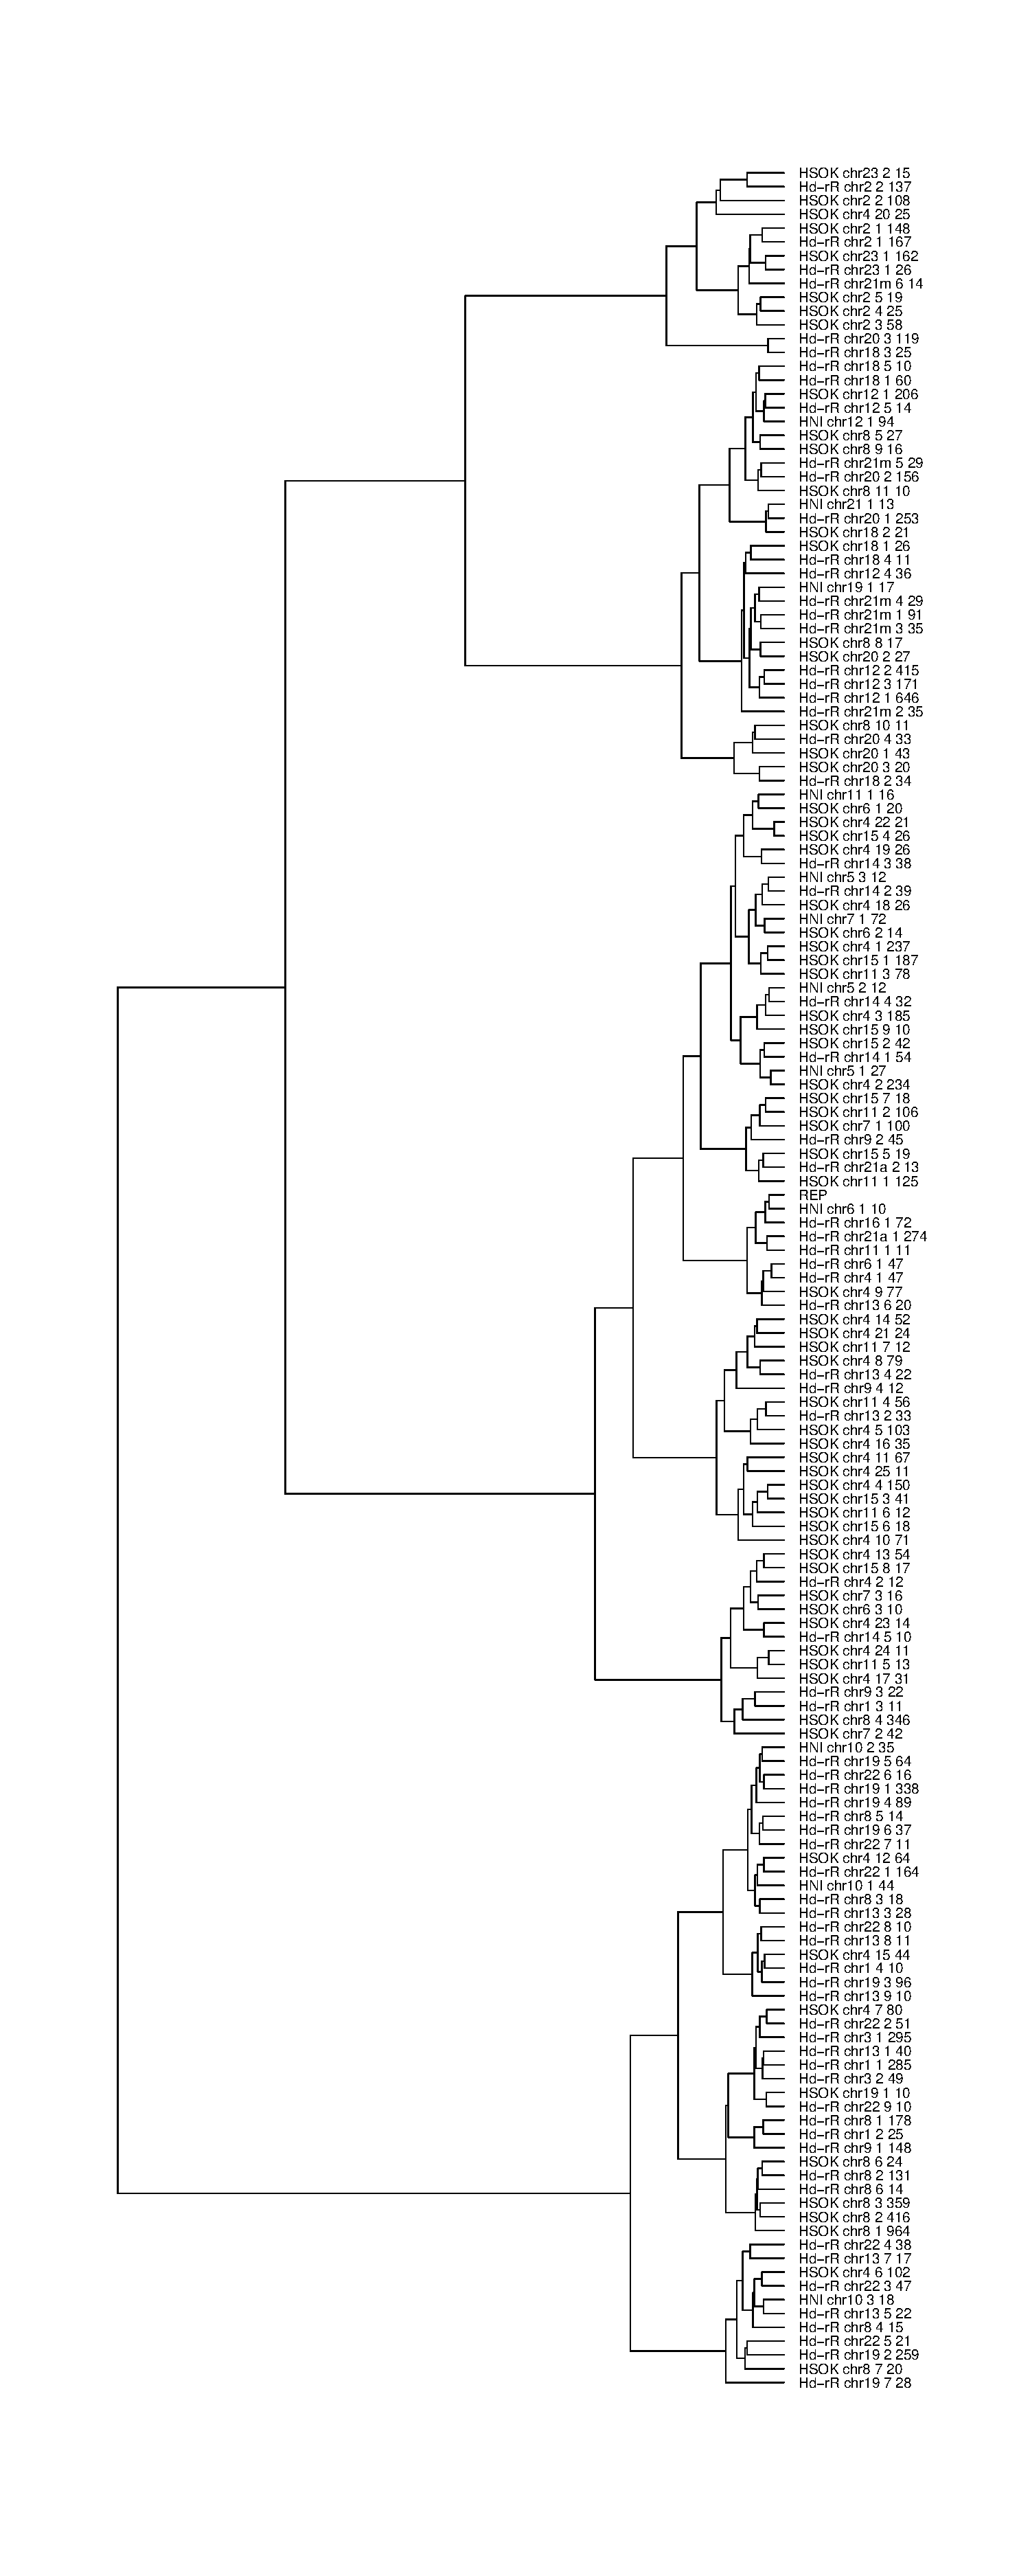
\includegraphics[width=0.5\linewidth]{representative_monomers_clustering.pdf}
  \caption{
    Hierarchical clustering of chromosome-representative monomers. Monomers are labeled as species, chromosome, cluster index, number of the cluster constituents.
  }
\end{figure*}

\begin{table*}
  \centering
  \caption{Super-chromosomal subfamilies of centromeric repeats}
  \begin{tabular}{p{0.6cm}p{3.4cm}p{1.5cm}p{2cm}p{4.5cm}p{3.7cm}}
  \hline
  SF & Hd-rR & HNI & HSOK & combined & positions \\ \hline
  1 & 4,6,9,11,14,16,21a (1,13) & 5,6,7,11    & 4,6,7,11,15 (8) & 4,5,6,7,9,11,14,15,16,21a (1,8,13) & 1M+1SM+14A (2SM+1A) \\
  2 & 1,3,8,9,13,19,22          & 10          & 8,19 (4)        & 1,3,8,9,10,13,19,22 (4)            & 6SM+2ST+2A (1M) \\
  3 & 12,18,20,21m (8)          & 12,21 (19)  & 12,18,20 (8)    & 12,18,20,21m (8,19)                & 1M+8SM+2ST+1A (2SM) \\
  4 & 2,23 (21m)                &             & 2,23 (4)        & 2,23 (4,21m)                       & 3M+1SM (2M) \\
  \hline
\end{tabular}

  \label{super_chromosomal_subfamiy}
  \caption*{{\small
    Chromosomes were classified into four subfamilies (SF). Chromosomes in brackets are the ones that have significantly more amount of repeats classified into another subfamily. Hd-rR chromosome 21 possessed two distantly-positioned arrays, thus is notated as 21m (metacentric) and 21a (acrocentric; see Table \ref{centromeric_repeat_distribution} for detail). Summarizing the chromosomes from the three strains, 22 out of the 24 chromosomes were assigned to one or two subfamilies. Notation of the centromeric positions are the same as Table \ref{centromeric_repeat_distribution}.
  }}
\end{table*}
